% Simulation-to-robot pipeline (Chapter 6, sec:preliminary_sim_methods).
% Compile: pdflatex -output-directory=.. pipeline.tex
% Hardware data flow per the dissertation text: the SNS network is evaluated
% on the Jetson Orin, which commands the Teensy-class MCUs; the MCUs close
% the per-joint valve, pressure, and contact loops on the biped. The
% computer-in-the-loop note sits under the bands, clear of all lines.
\documentclass[border=6pt]{standalone}
\usepackage[T1]{fontenc}
\usepackage{mathpazo}
\usepackage{tikz}
\usetikzlibrary{arrows.meta, positioning, calc, fit}
\begin{document}
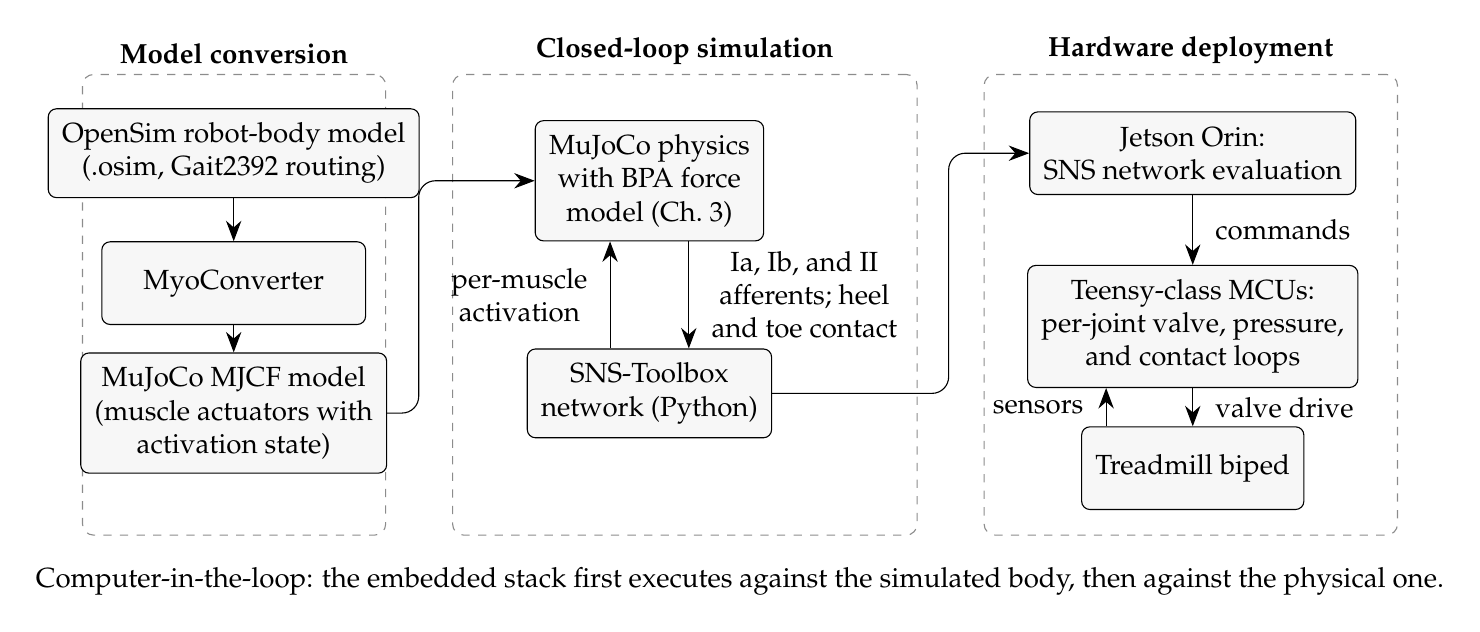
\begin{tikzpicture}[
  font=\normalsize,
  box/.style={draw, rounded corners=3pt, align=center, inner sep=5pt,
              minimum height=1.05cm, fill=black!3},
  arrow/.style={-{Stealth[length=2.6mm]}, thin, rounded corners=6pt},
  lab/.style={align=center, inner sep=3pt},
  band/.style={draw=black!45, dashed, rounded corners=4pt, inner sep=0pt},
  head/.style={align=center, font=\normalsize\bfseries},
]

% ---- Phase bands
\node[band, fit={(0.30,0) (4.15,-5.85)}, label={[head]above:Model conversion}] (b1) {};
\node[band, fit={(5.00,0) (10.90,-5.85)}, label={[head]above:Closed-loop simulation}] (b2) {};
\node[band, fit={(11.75,0) (17.00,-5.85)}, label={[head]above:Hardware deployment}] (b3) {};

% ---- Phase 1: conversion chain
\node[box, minimum width=3.35cm] (osim) at (2.22,-1.0)  {OpenSim robot-body model\\(.osim, Gait2392 routing)};
\node[box, minimum width=3.35cm] (myoc) at (2.22,-2.65) {MyoConverter};
\node[box, minimum width=3.35cm] (mjcf) at (2.22,-4.30) {MuJoCo MJCF model\\(muscle actuators with\\activation state)};
\draw[arrow] (osim) -- (myoc);
\draw[arrow] (myoc) -- (mjcf);

% ---- Phase 2: closed loop, orthogonal exchange with margin labels
\node[box, minimum width=2.9cm] (phys) at (7.5,-1.35) {MuJoCo physics\\with BPA force\\model (Ch.~3)};
\node[box, minimum width=2.9cm] (sns) at (7.5,-4.05) {SNS-Toolbox\\network (Python)};
\draw[arrow] ($(sns.north)+(-0.5,0)$) -- ($(phys.south)+(-0.5,0)$)
  node[lab, midway, left=5pt] {per-muscle\\activation};
\draw[arrow] ($(phys.south)+(0.5,0)$) -- ($(sns.north)+(0.5,0)$)
  node[lab, midway, right=5pt] {Ia, Ib, and II\\afferents; heel\\and toe contact};

% ---- Phase 3: hardware stack (Jetson evaluates, MCUs drive)
\node[box] (jetson) at (14.40,-1.00) {Jetson Orin:\\SNS network evaluation};
\node[box] (teensy) at (14.40,-3.20) {Teensy-class MCUs:\\per-joint valve, pressure,\\and contact loops};
\node[box] (biped) at (14.40,-5.00) {Treadmill biped};
\draw[arrow] (jetson) -- node[lab, right=5pt] {commands} (teensy);
\draw[arrow] (teensy) -- node[lab, right=5pt] {valve drive} (biped);
\draw[arrow] ($(biped.north)+(-1.1,0)$) -- node[lab, left=5pt] {sensors} ($(teensy.south)+(-1.1,0)$);

% ---- Cross-phase connectors through the band gutters
\draw[arrow] (mjcf.east) -- ++(0.40,0) |- (phys.west);
\draw[arrow] (sns.east) -- (11.30,-4.05) |- (jetson.west);

% ---- Note under the bands
\node[lab, anchor=north] at (8.65,-6.15)
  {Computer-in-the-loop: the embedded stack first executes against the simulated body, then against the physical one.};

\end{tikzpicture}
\end{document}
